\documentclass[conference,a4paper,english]{IEEEtran}

\usepackage{babel}
\usepackage[cmex10]{amsmath}
\usepackage{amssymb}
\usepackage{tgpagella}
\usepackage{fontspec}
\usepackage{unicode-math}
\setmainfont[Ligatures=TeX]{TeX Gyre Pagella}
\setsansfont[Ligatures=TeX]{TeX Gyre Heros}
\setmonofont[Scale=0.9]{TeX Gyre Cursor}
\setmathfont[Ligatures=TeX]{TeX Gyre Pagella Math}
\usepackage[official]{eurosym}
\usepackage{graphicx}
\graphicspath{{./img/}}
\usepackage{booktabs}
\usepackage{multirow}
\usepackage{ragged2e}
\usepackage{csquotes}
\usepackage{flushend} 
\usepackage{hologo}
\usepackage[backend=biber,%
  hyperref,%
  alldates=iso8601,%
  %backref,%
  %backrefstyle=none,%
  style=numeric,%
  sorting=nyt,%
]{biblatex}
\ExecuteBibliographyOptions{doi=false,url=false}
\newbibmacro{string+doiurlisbn}[1]{%
  \iffieldundef{doi}{%
    \iffieldundef{url}{%
      \iffieldundef{isbn}{%
        \iffieldundef{issn}{%
          #1%
        }{%
          \href{https://books.google.com/books?vid=ISSN\thefield{issn}}{#1}%
        }%
      }{%
        \href{https://books.google.com/books?vid=ISBN\thefield{isbn}}{#1}%
      }%
    }{%
      \href{\thefield{url}}{#1}%
    }%
  }{%
    \href{http://dx.doi.org/\thefield{doi}}{#1}%
  }%
}
\DeclareFieldFormat*{title}{\usebibmacro{string+doiurlisbn}{\mkbibquote{#1}}}

\bibliography{../bibliography.bib}
\usepackage[group-digits=integer,%
  group-minimum-digits=4,%
  list-final-separator={, and },%
  add-integer-zero=false,%
  free-standing-units,%
  unit-optional-argument,%
  binary-units,%
  detect-weight=true,%
  detect-inline-weight=math,%
]{siunitx}
%\SendSettingsToPgf
\usepackage{minted}
\setminted{%
  autogobble,%
  breaklines=true,%
  fontsize=\small,%
  linenos=false,%
  %xleftmargin=2em,%
  %xrightmargin=2em,%
}
\usepackage{paralist}
\usepackage{microtype}
\usepackage[dvipsnames]{xcolor}
\definecolor{halfgray}{gray}{0.55}
\definecolor{webgreen}{rgb}{0,0.5,0}
\definecolor{webbrown}{rgb}{.6,0,0}
\definecolor{thesisblue}{cmyk}{1.00,0.50,0.10,0.01}
\usepackage{hyperref}
\hypersetup{%
  colorlinks=true,%
  breaklinks=true,%
  linktocpage=true,%
  pdfstartview=FitV,%
  pdfpagemode=UseNone,%
  pdfpagemode=UseOutlines,%
  plainpages=false,%
  bookmarksnumbered,%
  hypertexnames=true,%
  pdfhighlight=/0,%
  urlcolor=webbrown,%
  linkcolor=thesisblue,%
  citecolor=webgreen,%
  pdftitle={A Beginner's Guide to Scientific Data Presentation using LaTeX},%
  pdfauthor={Stephan Lukasczyk},%
  pdfkeywords={siunitx, booktabs, data, presentation, latex, r, sweave,
    pstricks, pgfplots, lua}
  pdfsubject={},%
}

\newcommand\toolname[1]{\textsf{#1}}

\begin{document}

\title{A Beginner's Guide to Scientific Data Presentation using \LaTeX}

\author{\IEEEauthorblockN{Stephan Lukasczyk}
  \IEEEauthorblockA{IEEE Student Branch Passau\\
    94032 Passau, Germany\\
    \href{mailto:tex@lukasczyk.me}{tex@lukasczyk.me}}}

\maketitle

% As a general rule, do not put math, special symbols or citations
% in the abstract
\begin{abstract}
  Evaluating the work done for a seminar paper, a thesis, or even a scientific
  publication often forces students to present a large amount of data in a
  consistent and appropriate way.  Doing so, one will encounter many pitfalls
  due to the complexity of the task.  It can be a long-running and frustrating
  process to find out, which way works the best.  Although, we cannot provide
  universally valid rules, we want to give some hints and guidelines with this
  work.  Therefore, we present formal aspects, packages and tools, that are
  helpful when presenting the evaluation results and data in general.

  Our tools of choice are all from the \LaTeX{} universe; obviously, the formal
  aspects of data presentation are valid for other tools as well.  We show a
  variety of \LaTeX{} packages and give an introduction into their usage, in
  order to show how easy the presentation of data can be.

  Only a small knowledge of \LaTeX{} is needed to understand the source
  examples, as we try to provide all examples in a very simple and
  self-explaining way.
\end{abstract}
\begin{IEEEkeywords}
  siunitx, booktabs, data, presentation, latex, r, sweave, pstricks, pgfplots,
  lua
\end{IEEEkeywords}

\section{Motivation}

When evaluating an experiment, one usually has to deal with a large amount of
data.  After deciding, which data should be discussed in the evaluation part of
a seminar paper or a thesis, the main problem is \emph{how} to present this
data. Obviously, one will choose use tables, plots, or other kinds of figures.
Finding out, which type of presentation is the best, depends on the own point of
view; thus, it will not be part of this work.

We will focus on the different ways of presenting the data.  In order to achieve
this, we will use \LaTeX\@.  We show several packages and how to use them; we
also show some tools, e.g., to easily create plots of the data.  Additionally,
we provide some ways to automatically process the data, in order to minimize the
amount of work that needs to be done manually.  The reason for the latter is to
avoid a complex and error-prone processing work flow.

All source code of the examples, as well as of this paper and the presentation,
can be found on GitHub\footnote{%
  \href{https://github.com/IEEE-SB-Passau/latex-data-presentation}%
    {https://github.com/IEEE-SB-Passau/latex-data-presentation}}; on a
supplementary web page\footnote{%
  \href{https://research.lukasczyk.me/latex-data-presentation}%
    {https://research.lukasczyk.me/latex-data-presentation}} we also provide all
examples, both the source code and the compiled results.

In order to understand the examples, it's not necessary to be a professional
\LaTeX{} user.  We try to provide very simple examples that are
self-explanatory.  Although, we restrict our presentation to \LaTeX{}, the rules
are valid in a general context and can be applied to every other typesetting
tool of your choice.  For a deeper introduction into \LaTeX{}, we suggest the
German book \enquote{Einführung in \LaTeX} by Herbert Voß~\cite{Voss2012} or the
well-known \enquote{\hologo{LaTeX2e}-Kurzbeschreibung} by Marco Daniel et
al~\cite{Daniel2015}.  An English introduction can be found in \enquote{The Not
So Short Introduction to \hologo{LaTeX2e}} by Tobias Oetiker et
al~\cite{Oetiker2015}; a more comprehensive work is \enquote{The \LaTeX{}
Companion} by Frank Mittelbach et al~\cite{Mittelbach2008}.


\section{Presenting Numbers}

Before we dig into the possibilities of presenting data, we want to give some
general advice about numbers.  When presenting data, almost all is about
numbers; it makes an obvious difference, if a number is presented like
$648312786157.546863$ or \num{648312786157.546863}.  With the former it is hard
to determine the dimension of this number, while it is easy with the latter.

A general advice is to group numbers with four or more digits; whether a small
space~(\mintinline{latex}{\,} in \LaTeX), a comma or a dot is used, depends on
the language, country and personal taste; in Germany, the comma is the decimal
mark, while in English it is the dot.  The German norms DIN~1333 and DIN~5008
state that only a small space should be used for grouping; they are only allowed
money amounts.  In English speaking countries one can use a small space or a
comma for grouping.

\subsection{Units}

When presenting results, the numbers should be consistent in terms of units and
their significance; most of the information in this and the following section is
taken from Beyer, Löwe, and Wendler~\cite{BeyerLoeweWendler2016}.  The first and
most general recommendation is to use SI units; an exception of this rule are
time intervals, where the hours or even days are preferable over seconds.

In Computer Science, we often measure in bytes.  The prefixes \emph{kilo} (k),
\emph{mega} (M), \emph{giga} (G) etc.\ are SI prefixes, that means, they always
represent a factor of \num{1000}.  Because of the binary nature of computers, we
sometimes want to use the factor \num{1024} instead; if we do so, the prefixes
\emph{kibi} (KiB), \emph{mibi} (MiB), \emph{gibi} (GiB), etc.\ need to be used.
Be aware of the different basis, which will lead to an error in precision if
used wrong: with the prefix mega it would be \SI{4.9}{\percent} and
\SI{7.4}{\percent} with giga, respectively—a significant error.

\subsection{Significant Digits}

\subsection{The Package \toolname{siunitx}}

In order to get the number formatting right, a number of packages evolved; most
known is the \toolname{siunitx} package by Joseph Wright~\cite{Wright2016}.  It
was designed for formatting physical quantities and therefore as a much richer
functionality than we need.

When using the command in Listing~\ref{lst:siunitx-options} to load the package,
all things mentioned above are set correctly.

\begin{listing}[H]
\begin{minted}{latex}
\usepackage[group-digits=integer,%
  group-minimum-digits=4,%
  list-final-separator={, and },%
  add-integer-zero=false,%
  free-standing-units,%
  unit-optional-argument,%
  binary-units,%
  detect-weight=true,%
  detect-inline-weight=math,%
]{siunitx}
\end{minted}
\caption{Suggested options when loading \toolname{siunitx}}
\label{lst:siunitx-options}
\end{listing}

With these settings, all numbers enclosed in all \toolname{siunitx} commands
like \mintinline{latex}{\num{}}, \mintinline{latex}{\numlist{}},
\mintinline{latex}{\SI{}{}} will be formatted the
following way:
\begin{itemize}
  \item only the integer numbers will be grouped, that means, the part left of a
    decimal dot
  \item this is only done if the number has at least four digits.
  \item in a \mintinline{latex}{\numlist}, the last number will be separated
    with \enquote{, and }, e.g. \numlist{5;10;42}
    (\mintinline{latex}{\numlist{5;10;42}}).
  \item if we omit the zero before a decimal dot, it will not be added
    automatically~(e.g. \num{.0815} in contrast to
    \num[add-integer-zero=true]{.0815})
  \item the unit macros like \mintinline{latex}{\second} exist also outside of
    \mintinline{latex}{\si} and \mintinline{latex}{\SI}
  \item these macros have an optional argument, so
    \mintinline{latex}{\SI{10}{\second}} and \mintinline{latex}{\second[10]}
    both produce the output \second[10].
  \item the prefixes \emph{kibi}, \emph{mibi} and so on are available, together
    with \mintinline{latex}{\bit} and \mintinline{latex}{\byte}
  \item \toolname{siunitx} will detect the font weight from the context
\end{itemize}

For a detailed explanation of the options and all other available options of the
\toolname{siunitx} package, we refer the reader to the package
documentation~\cite{Wright2016}.


\section{Tables}

\subsection{General Rules}

\subsection{Tuning}


\section{How to Create Plots?}

We will now show several possibilities for plotting, using different
technologies. For each of the following technologies, we give an example to
provide an idea to the reader of how the work with this technology might look
like. The examples are in alphabetical order of the technology name; afterwards
we will only look closer into \texttt{pgfplots}.

\subsection{Gnuplot}

\toolname{Gnuplot} is a portable command-line driven graphing utility for
various platforms.  It is freely available under a free license.  Originally
created in 1986, it is a tool that allows the user to visualize mathematical
functions and data interactively~\cite{WilliamsKelley2016}.  The documentation
and many examples can be found on the project's
homepage\footnote{\href{http://www.gnuplot.info}{http://www.gnuplot.info}}.

\toolname{Gnuplot} can produce its output in many different formats: directy on
screen, or as graphics file, include PNG, EPS, SVG, JPEG, and many more; it is
also capable of producing \LaTeX{} code that can be included directly in
\LaTeX{} documents.

\subsection{pgfplots}

\toolname{Pgfplots} is a package for \TeX{} and \LaTeX{} using Till Tantau's
package \toolname{pgf/Ti\textit{k}Z}~\cite{Feuersaenger2016}.  It supports line
plots, scatter plots, bar plots, histogram plots, box plots, and many more and
is able to do 2D and 3D plots without needing an external tool installed
(contrary to \toolname{PSTricks}).

The input file is of the structure as a standard \TeX{} or \LaTeX{} file.
Consider the example code in Listing~\ref{lst:pgfplots-example}, which is taken
from the \toolname{pgfplots} manual~\cite{Feuersaenger2016}.  It uses a data set
that comes with \toolname{pgfplots} to plot the curve that can be seen in
Figure~\ref{fig:pgfplots-example}.

\begin{listing}[H]
  \inputminted{latex}{../examples/pgfplots-example.tex}
  \caption{Example code for \toolname{pgfplots} (taken
    from~\cite{Feuersaenger2016})}
  \label{lst:pgfplots-example}
\end{listing}
\begin{figure}[!t]
  \centering
  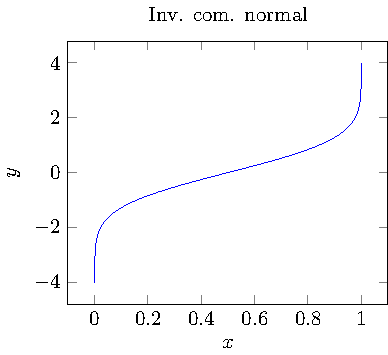
\includegraphics{pgfplots-example}
  \caption{Resulting diagram from the code in Lst.~\ref{lst:pgfplots-example}}
  \label{fig:pgfplots-example}
\end{figure}

\subsection{PSTricks}

\subsection{R and Sweave}

\toolname{R} is a well-known language for statistical computing and
graphics~\cite{Ihaka1998}.  A huge variety of modules is available at the
Comprehensive R Archive Network (CRAN)\footnote{%
  \href{https://cran.r-project.org}{https://cran.r-project.org}}.  One of these
modules is called \toolname{Sweave}, initially developed by Friedrich
Leisch~\cite{Leisch2002}.  It combines \LaTeX{} and \toolname{R} in the style of
literate programming—a concept developed by Donald E\@. Knuth~\cite{Knuth1992}.
A simple introduction was given by Uwe Ziegenhagen in his German article
\enquote{Datenanalyse mit Sweave, \LaTeX{} und R}~\cite{Ziegenhagen2010}.

In order to use \toolname{Sweave}, one needs to write a document like shown in
Listing~\ref{lst:sweave-example}.  By convention, the filename suffix is not
\texttt{*.tex} but \texttt{*.Snw}; this is important, because the \texttt{*.tex}
file will be create automatically.  A syntax highlighting mode is available for
the editor VIM\@.  After writing the file, one needs to start \toolname{R},
e.g., a \toolname{R} interactive shell.  With the command
\mintinline{R}{Sweave("filename.Snw")} the \toolname{R} code will be processed
and a \texttt{*.tex} file will be created, which can then be processed by, e.g.,
\hologo{pdfLaTeX}.

The example in Listing~\ref{lst:sweave-example} loads the exchange rates between
\euro{} and \$ from the homepage of the European Central Bank and plots it. The
output can be seen in Figure~\ref{fig:sweave-example}.

\begin{listing}[H]
  \inputminted{latex}{../examples/sweave-example.Snw}
  \caption{Plot the exchange rate between \euro{} and \$ dynamically using
    \toolname{Sweave}}
  \label{lst:sweave-example}
\end{listing}
\begin{figure}[!t]
  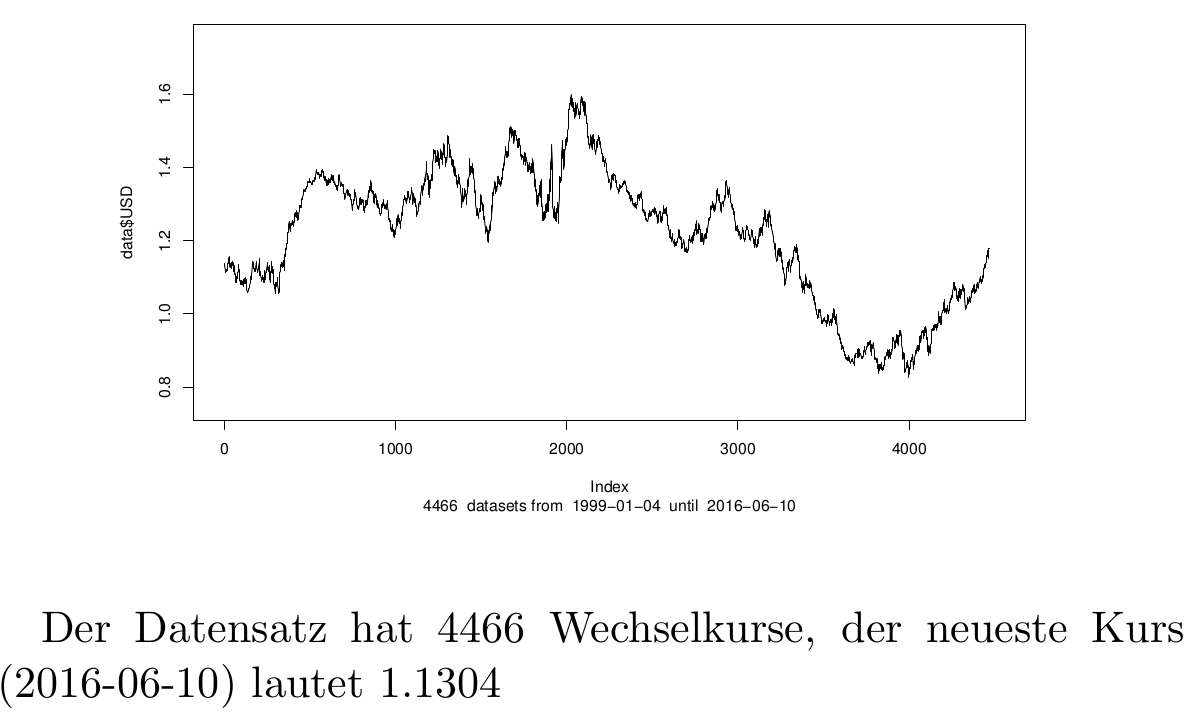
\includegraphics[width=\linewidth]{sweave-example}
  \caption{Screenshot of the \toolname{Sweave} example in
    Lst.~\ref{lst:sweave-example}}
  \label{fig:sweave-example}
\end{figure}


\section{Plots}

In this section, we want to focus on different examples of plots.  We restrict
our presentation to \toolname{pgfplots} because it is the tool we use most;
every example can be done with the other tools, respectively.  The raw data that
is used in the examples can be found in the supplementary GitHub
repository\footnoteref{footnote-github} and on the supplementary web
page\footnoteref{footnote-webpage}.


\section{Summary}

With this work, we have given a short overview over the possibilities of data
presentation in a scientific environment using \hologo{LaTeX}.  We gave hints on
the presentation of numbers and units using the package \toolname{siunitx}.  We
also made the reader aware of the importance of significant digits as well as
the differences between English and German typesetting of numbers.

We continued on tables and gave some general rules of designing tables: use
rules as spare as possible and avoid vertical lines completely!  The
\toolname{booktabs} package provides additional macros for the design of tables.
We also focused on number presentation within tables with the help of the
\toolname{siunitx} package.

Afterwards we introduced some tools to create plots: \toolname{Gnuplot},
\toolname{pgfplots}, \toolname{PSTricks}, and \toolname{R/Sweave}.  Finally, we
concluded with some examples on different plotting types using the
\toolname{pgfplots} package.

Furthermore, we provided a large number of literature and references to the
reader for further studies of the topic.


% trigger a \newpage just before the given reference
% number - used to balance the columns on the last page
% adjust value as needed - may need to be readjusted if
% the document is modified later
%\IEEEtriggeratref{8}
% The "triggered" command can be changed if desired:
%\IEEEtriggercmd{\enlargethispage{-5in}}

% references section

% can use a bibliography generated by BibTeX as a .bbl file
% BibTeX documentation can be easily obtained at:
% http://www.ctan.org/tex-archive/biblio/bibtex/contrib/doc/
% The IEEEtran BibTeX style support page is at:
% http://www.michaelshell.org/tex/ieeetran/bibtex/
%\bibliographystyle{IEEEtran}
% argument is your BibTeX string definitions and bibliography database(s)
%\bibliography{IEEEabrv,../bib/paper}
%
% <OR> manually copy in the resultant .bbl file
% set second argument of \begin to the number of references
% (used to reserve space for the reference number labels box)
\printbibliography

% that's all folks
\end{document}


